\begin{figure}[h]
    \centering
    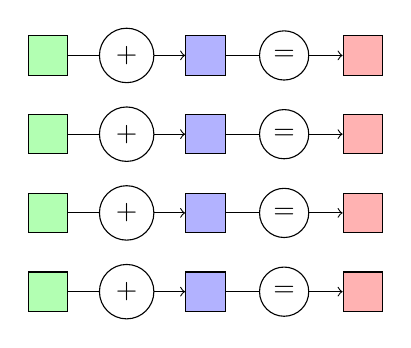
\begin{tikzpicture}

        \foreach \y in {0,..., 3}
            {
                \node[name=1_\y, draw, rectangle, minimum size=0.5cm, fill=green!30] at (0, \y) {};
                \node[name=2_\y, draw, rectangle, minimum size=0.5cm, fill=blue!30] at (2, \y) {};
                \node[name=3_\y, draw, rectangle, minimum size=0.5cm, fill=red!30] at (4, \y) {};
                \draw[->] (1_\y) -- node [circle, draw, fill=white] {$+$} (2_\y);
                \draw[->] (2_\y) -- node [circle, draw, fill=white] {$=$} (3_\y);
            }
    \end{tikzpicture}
    \caption{SISD Processing Example. One instruction is applied to each data item.}
    \label{fig:sisd}
\end{figure}